%!TEX root = ../Thesis.tex
\begin{figure}[h]
\centering
\begin{subfigure}[b]{0.45\textwidth}
    \centering
    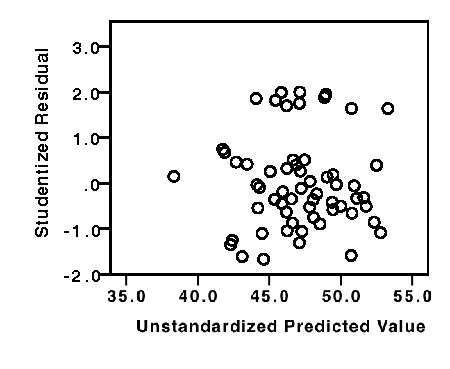
\includegraphics[width=\textwidth]{images/linearity/ValMax.eps}
    \caption{Related to test of valence, maximum pressure, and tap duration.}
    \label{fig:valence_maximum}
\end{subfigure}
\quad
\begin{subfigure}[b]{0.45\textwidth}
    \centering
    \includegraphics[width=\textwidth]{images/linearity/ValAvg.eps}
    \caption{Related to test of valence, average pressure, and tap duration.}
    \label{fig:valence_avg}
\end{subfigure}
\par\bigskip
\par\bigskip
\begin{subfigure}[b]{0.45\textwidth}
    \centering
    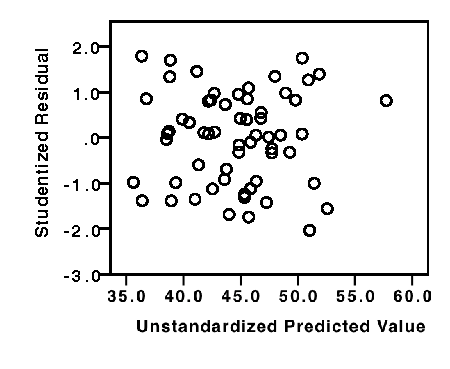
\includegraphics[width=\textwidth]{images/linearity/ArMax.eps}
    \caption{Related to test of arousal, maximum pressure, and tap duration.}
    \label{fig:arousal_maximum}
\end{subfigure}
\quad
\begin{subfigure}[b]{0.45\textwidth}
    \centering
    \includegraphics[width=\textwidth]{images/linearity/ArAvg.eps}
    \caption{Related to test of arousal, average pressure, and tap duration.}
    \label{fig:arousal_avg}
\end{subfigure}
\caption{Scatter plots of predicted values against studentized residuals. Note that because of randomness of data points, linearity can still be assumed. There is no indication of issues with homoscedasticity because there does not seem to be a funnel or fan shape.}
\end{figure}